%-*-    coding: UTF-8   -*-
% !TEX program = xelatex
\documentclass[UTF-8]{ctexart}
\usepackage{array}
\usepackage{graphicx}
\usepackage{float}
\usepackage{subfigure}
\usepackage{amsmath}
\usepackage{amssymb}
\usepackage{tabularx}
\usepackage{multirow}
\usepackage[usenames,dvipsnames]{color}
\usepackage{framed}
\usepackage{xcolor}
\usepackage{hyperref}
\usepackage{verbatim}
\hypersetup{
	colorlinks=true,
	linkcolor=black,
	filecolor=black,
	urlcolor=blue,
	citecolor=black,
}
\usepackage{ulem}
\usepackage[cache=false]{minted}
\setminted{tabsize=4}
\usepackage{geometry}
\geometry{a4paper,centering,scale=0.8}
\usepackage[format=hang,font=small,textfont=it]{caption}
\usepackage[nottoc]{tocbibind}

\definecolor{LightofNibel}{rgb}{0.6,0.85,0.95}
\pagecolor{white}

\title{\textbf{\huge 给信息组学弟学妹的 Linux 入门手把手教程}}
\author{\texttt{iotang}}
%\date{}

\begin{document}
	\maketitle
	
	\newpage
	
	\tableofcontents

	\newpage

	\section{欢迎使用 Linux!}
	
		学弟学妹们好!感谢你们参加信息学竞赛!
		
		比克提尼 iotang 在这里献上最诚挚的祝福!
		
		大家应该都对 Linux 有所耳闻,不过我猜有许多人都以为 Linux 很难用、不好用而不敢迈出第一步。
		
		其实,Linux 很好学,就如同你当年学 Windows 一样!
		
		其实,Linux 很好用,特别是对于你们“搞电脑的”而言!
		
		现在让 iotang 来手把手带领大家开启自己的 Linux 征程吧!
		
		~\\
		
		~\\
		
		\begin{figure}[H]
			\centering
			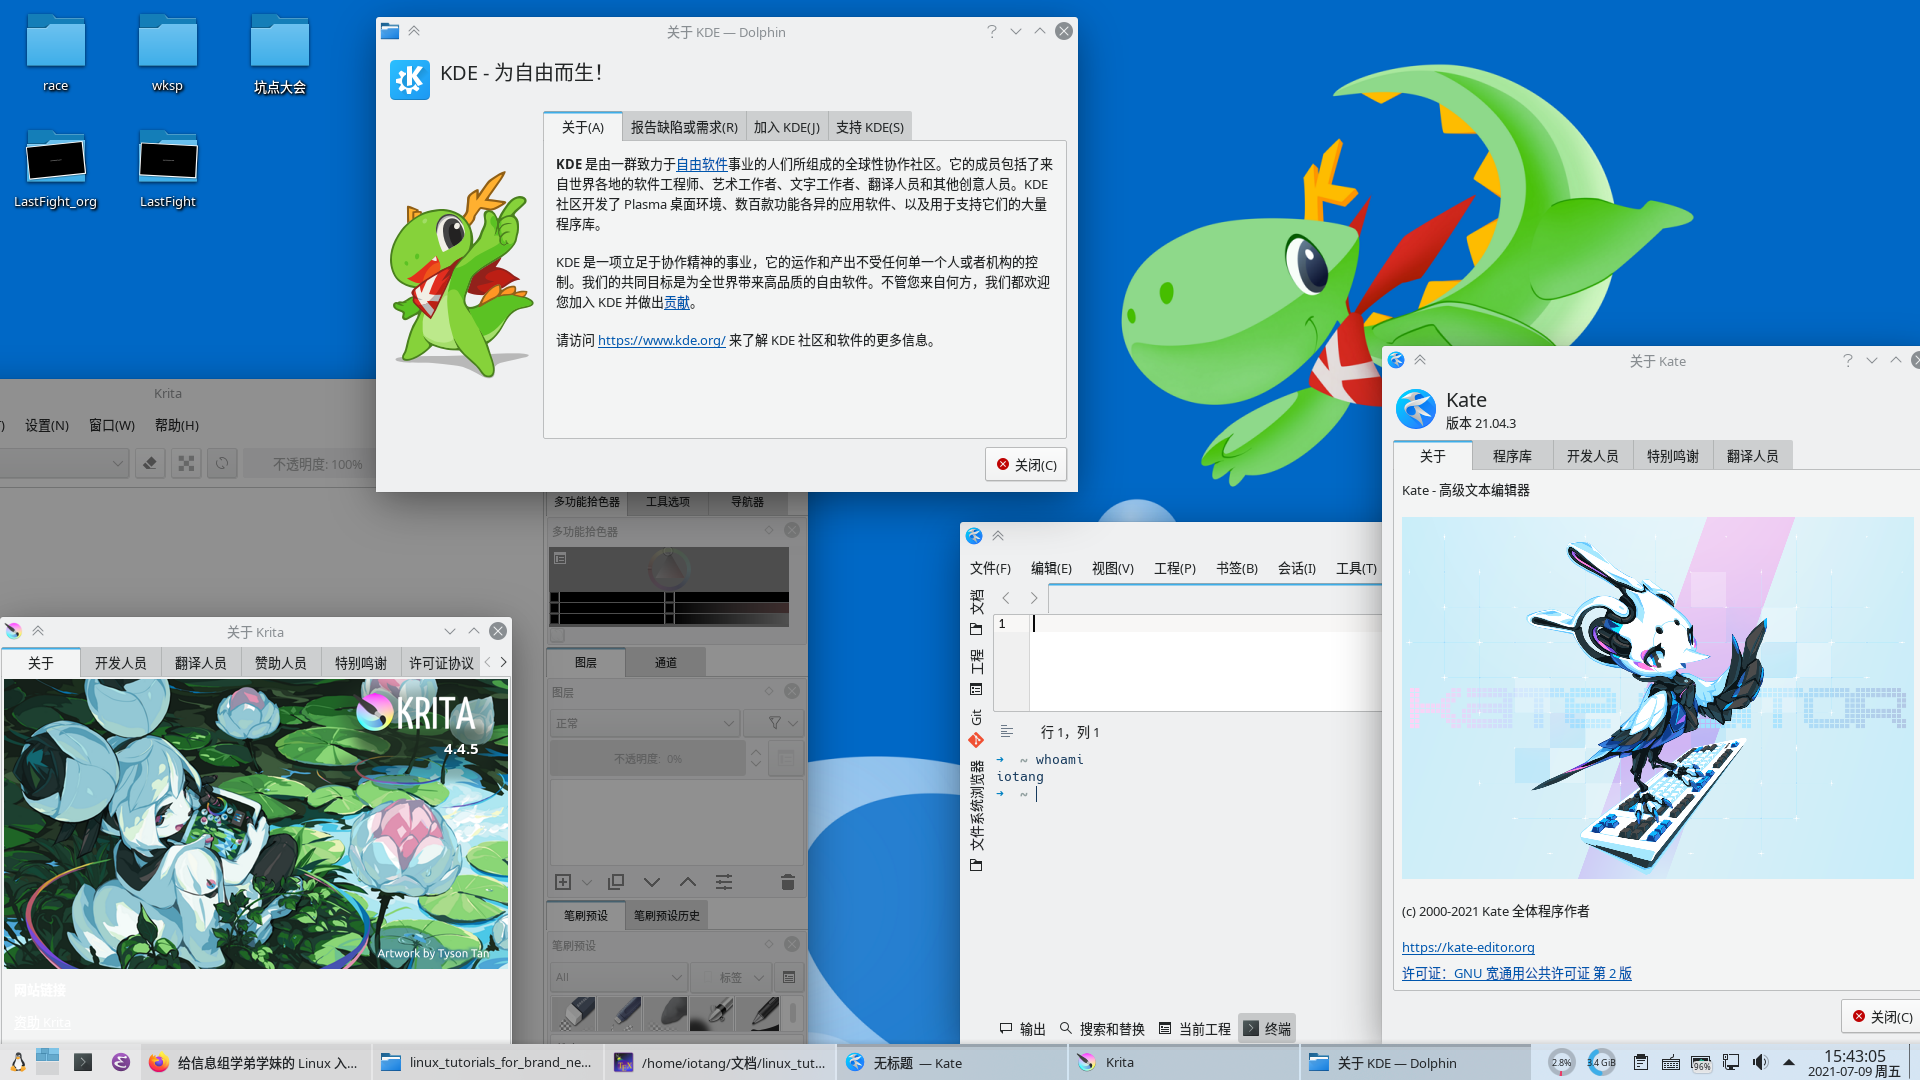
\includegraphics[width=0.8\textwidth]{fig/iotangsdesktop.png}
			\caption{iotang 的普普通通的 Arch Linux}
		\end{figure}
		
	\newpage
	
	\section{Linux 是开源软件}
	
		Linux 遵循 GNU 通用公共许可证,任何人都可以自由使用它的源代码。
		
		(注意,这里并没有说 Linux 是“不要钱”地使用的,不过既然你都可以搞到源代码了,那么收费基本也就没必要了。不过还是有服务以付费的方式给出。)
		
	\section{为什么是 Ubuntu?}
	
		接下来给大家带来的 Linux 教程主要是以 Ubuntu 为平台来实现的。
	
		首先很明显的是,NOI Linux 就是一个换皮的 Ubuntu。至于为什么是 Ubuntu,可能与 Ubuntu 在中国的强大的用户数量有关。
		
		用户多教程就多,问题解决也方便,\sout{不像笔者硬是要搞个 Arch Linux 然后折腾}。
		
		所以说,从竞赛与使用方面,这边还是建议大家用 Ubuntu。
	
	\newpage
	
	\section{Ubuntu 的安装}
	
		\subsection{搞到镜像文件}
		
			非常简单,你只要先百度 ubuntu,进入官网(注意:有中文官网),然后进入下载栏目下载就可以了。
			
			\subsubsection{我该选哪一个?}
			
				在下载界面你可以发现一些不同版本:
				
				\begin{figure}[H]
					\centering
					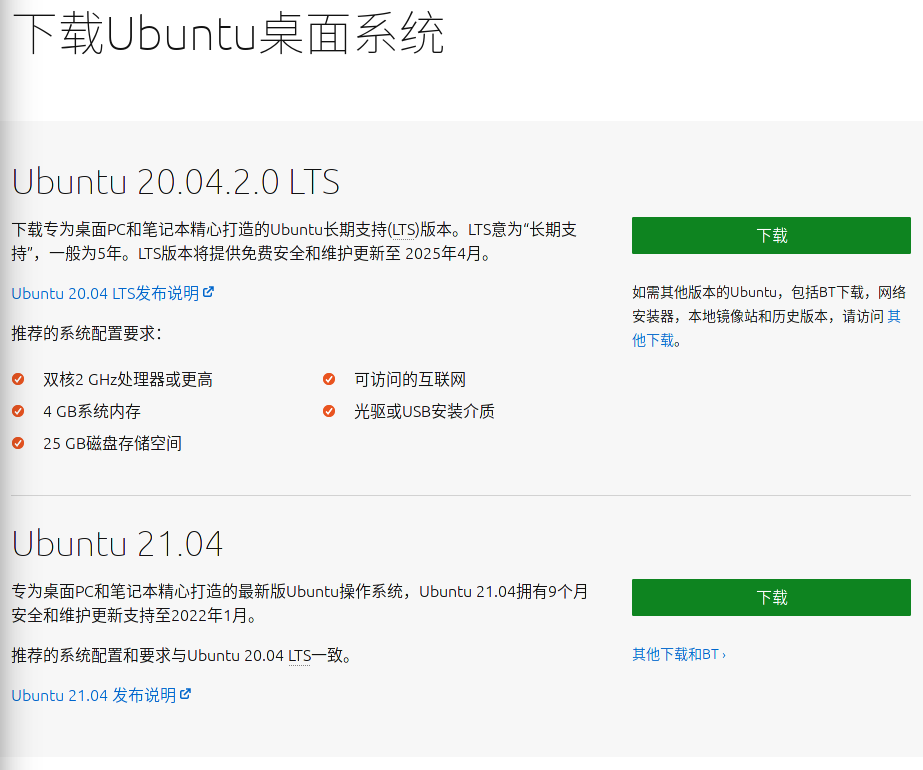
\includegraphics[width=0.8\textwidth]{fig/download_ubuntu_which.png}
					\caption{两种选择}
				\end{figure}
			
				其中,带“LTS”的版本意为长期支持版本,有 5 年的免费安全和维护更新时间;而不带 LTS 的一般只维护 9 个月(因为不带 LTS 的每半年发布一个,你需要及时更新)。
				
				这里为了稳定性,我们下载那个带 LTS 的版本。
			
			\subsubsection{下载的速度太慢了?}
			
				你可以去其它的镜像网站。这里以网易开源镜像站为例子:
				
				首先随便搜到它的主页。
				
				\begin{figure}[H]
					\centering
					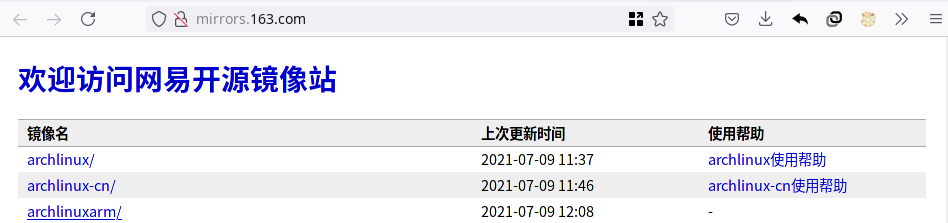
\includegraphics[width=0.8\textwidth]{fig/mirrors163com.png}
					\caption{http://mirrors.163.com/}
				\end{figure}
			
				然后找到 \texttt{ubuntu-releases}。
				
				\begin{figure}[H]
					\centering
					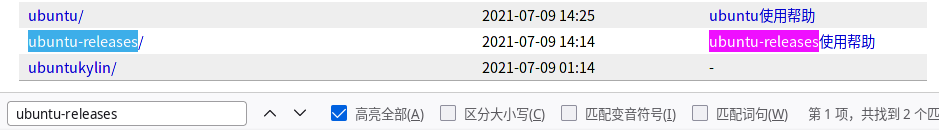
\includegraphics[width=0.8\textwidth]{fig/mirrors163com_find.png}
					\caption{找到 ubuntu-releases}
				\end{figure}
				
				然后选择正确的版本。
				
				\begin{figure}[H]
					\centering
					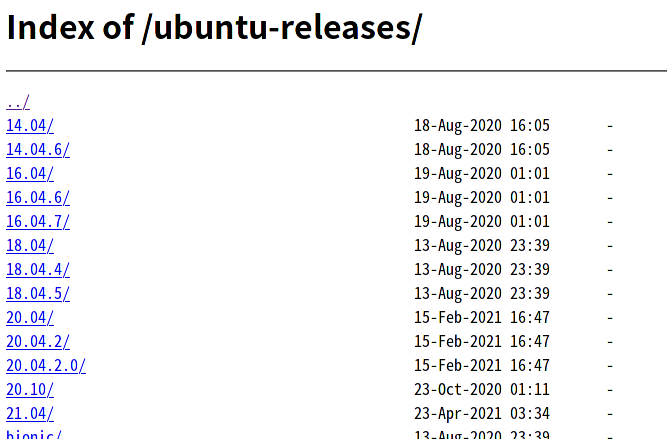
\includegraphics[width=0.8\textwidth]{fig/mirrors163com_in_ubuntu-releases.png}
					\caption{/ubuntu-releases/}
				\end{figure}
			
				下载桌面版,即名字里面有 desktop 的那个。
				
				\begin{figure}[H]
					\centering
					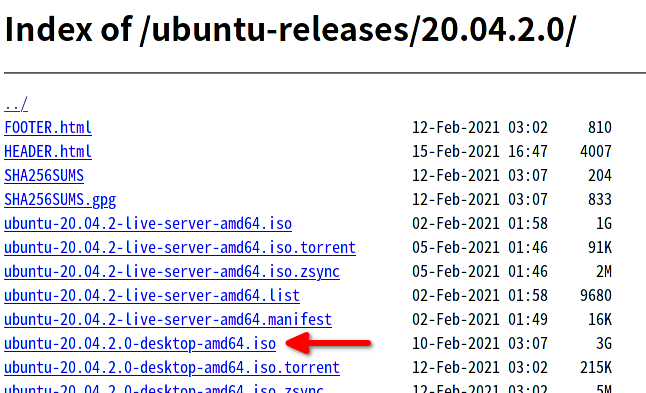
\includegraphics[width=0.8\textwidth]{fig/mirrors163com_choose_ubuntu-releases.png}
					\caption{选择桌面版}
				\end{figure}
			
		\subsection{制作启动盘}
		
			\subsubsection{在 Linux 下}
			
				系统但凡是有点良心都会自带一个启动盘创建器。比如笔者的:
			
				\begin{figure}[H]
					\centering
					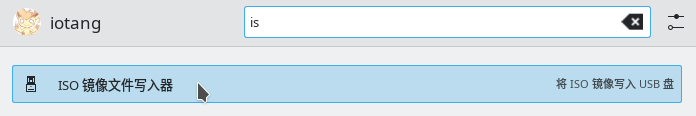
\includegraphics[width=0.8\textwidth]{fig/iso_burn.png}
					\caption{KDE 下的启动盘创建器}
				\end{figure}
				
				此时,你需要准备一个 U 盘(最好至少 8 GB,并且笔者建议这个 U 盘应该是空的,以确保\textbf{\large 没有重要文件在里面}被抹去。)
				
				启动盘创建器的用法基本都一样。注意不要选错 U 盘。
			
				\begin{figure}[H]
					\centering
					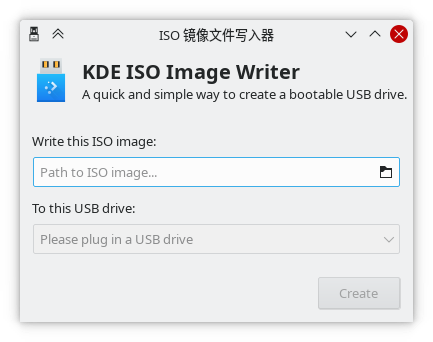
\includegraphics[width=0.3\textwidth]{fig/isoimagewriter.png}
					\caption{KDE 启动盘创建器}
				\end{figure}


			\subsubsection{在 Windows 下}
			
				去下载 Rufus 启动盘创建器。
				
				\begin{figure}[H]
					\centering
					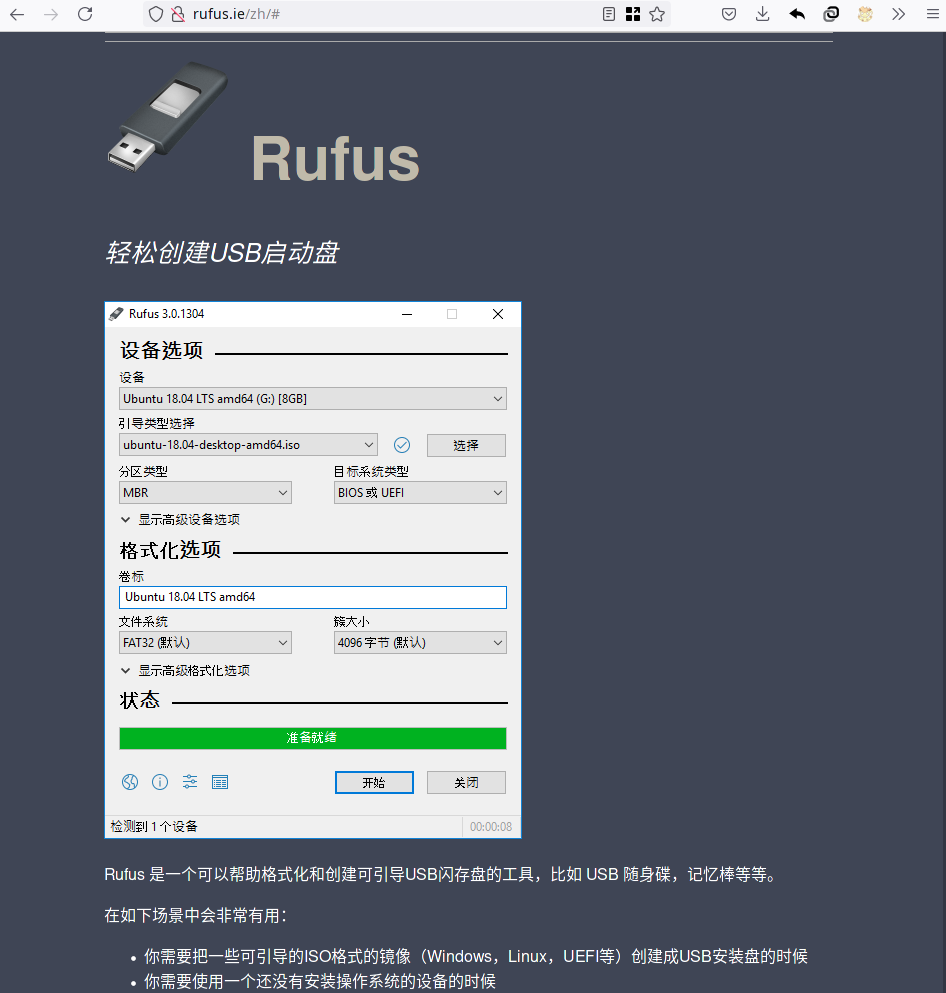
\includegraphics[width=0.8\textwidth]{fig/rufus.png}
					\caption{Rufus}
				\end{figure}
			
		\subsection{安装 Ubuntu}
		
			我们马上会在目标电脑(机房里面的一台)上安装 Ubuntu。
		
			\subsubsection{BIOS 设置}
			
				首先打开目标电脑,在 Logo 出现后(甚至从电源键按下前)开始狂按 BIOS 键(比如 F12、ESC、DEL 等等)。
				
				在 BIOS 设置中打开 U 盘启动,打开 UEFI 模式优先(原先一般是 Legacy 优先)。
			
			\subsubsection{启动}
				
				关机,插上启动盘,开机后会出来一个界面让你选择启动位置。选择你的 U 盘(一般叫 USB-HDD 什么的)。
				
				之后在 Try Ubuntu Without Installing 和 Install Ubuntu 中选择 Install Ubuntu。
				
				
	
\end{document}